


\section{Results}



\subsection{Previous Results}
Refer to previous results without binaries

Good fits to observables, strong BH constraints etc, show BH plots and list the contraints

\begin{figure}
	\centering
	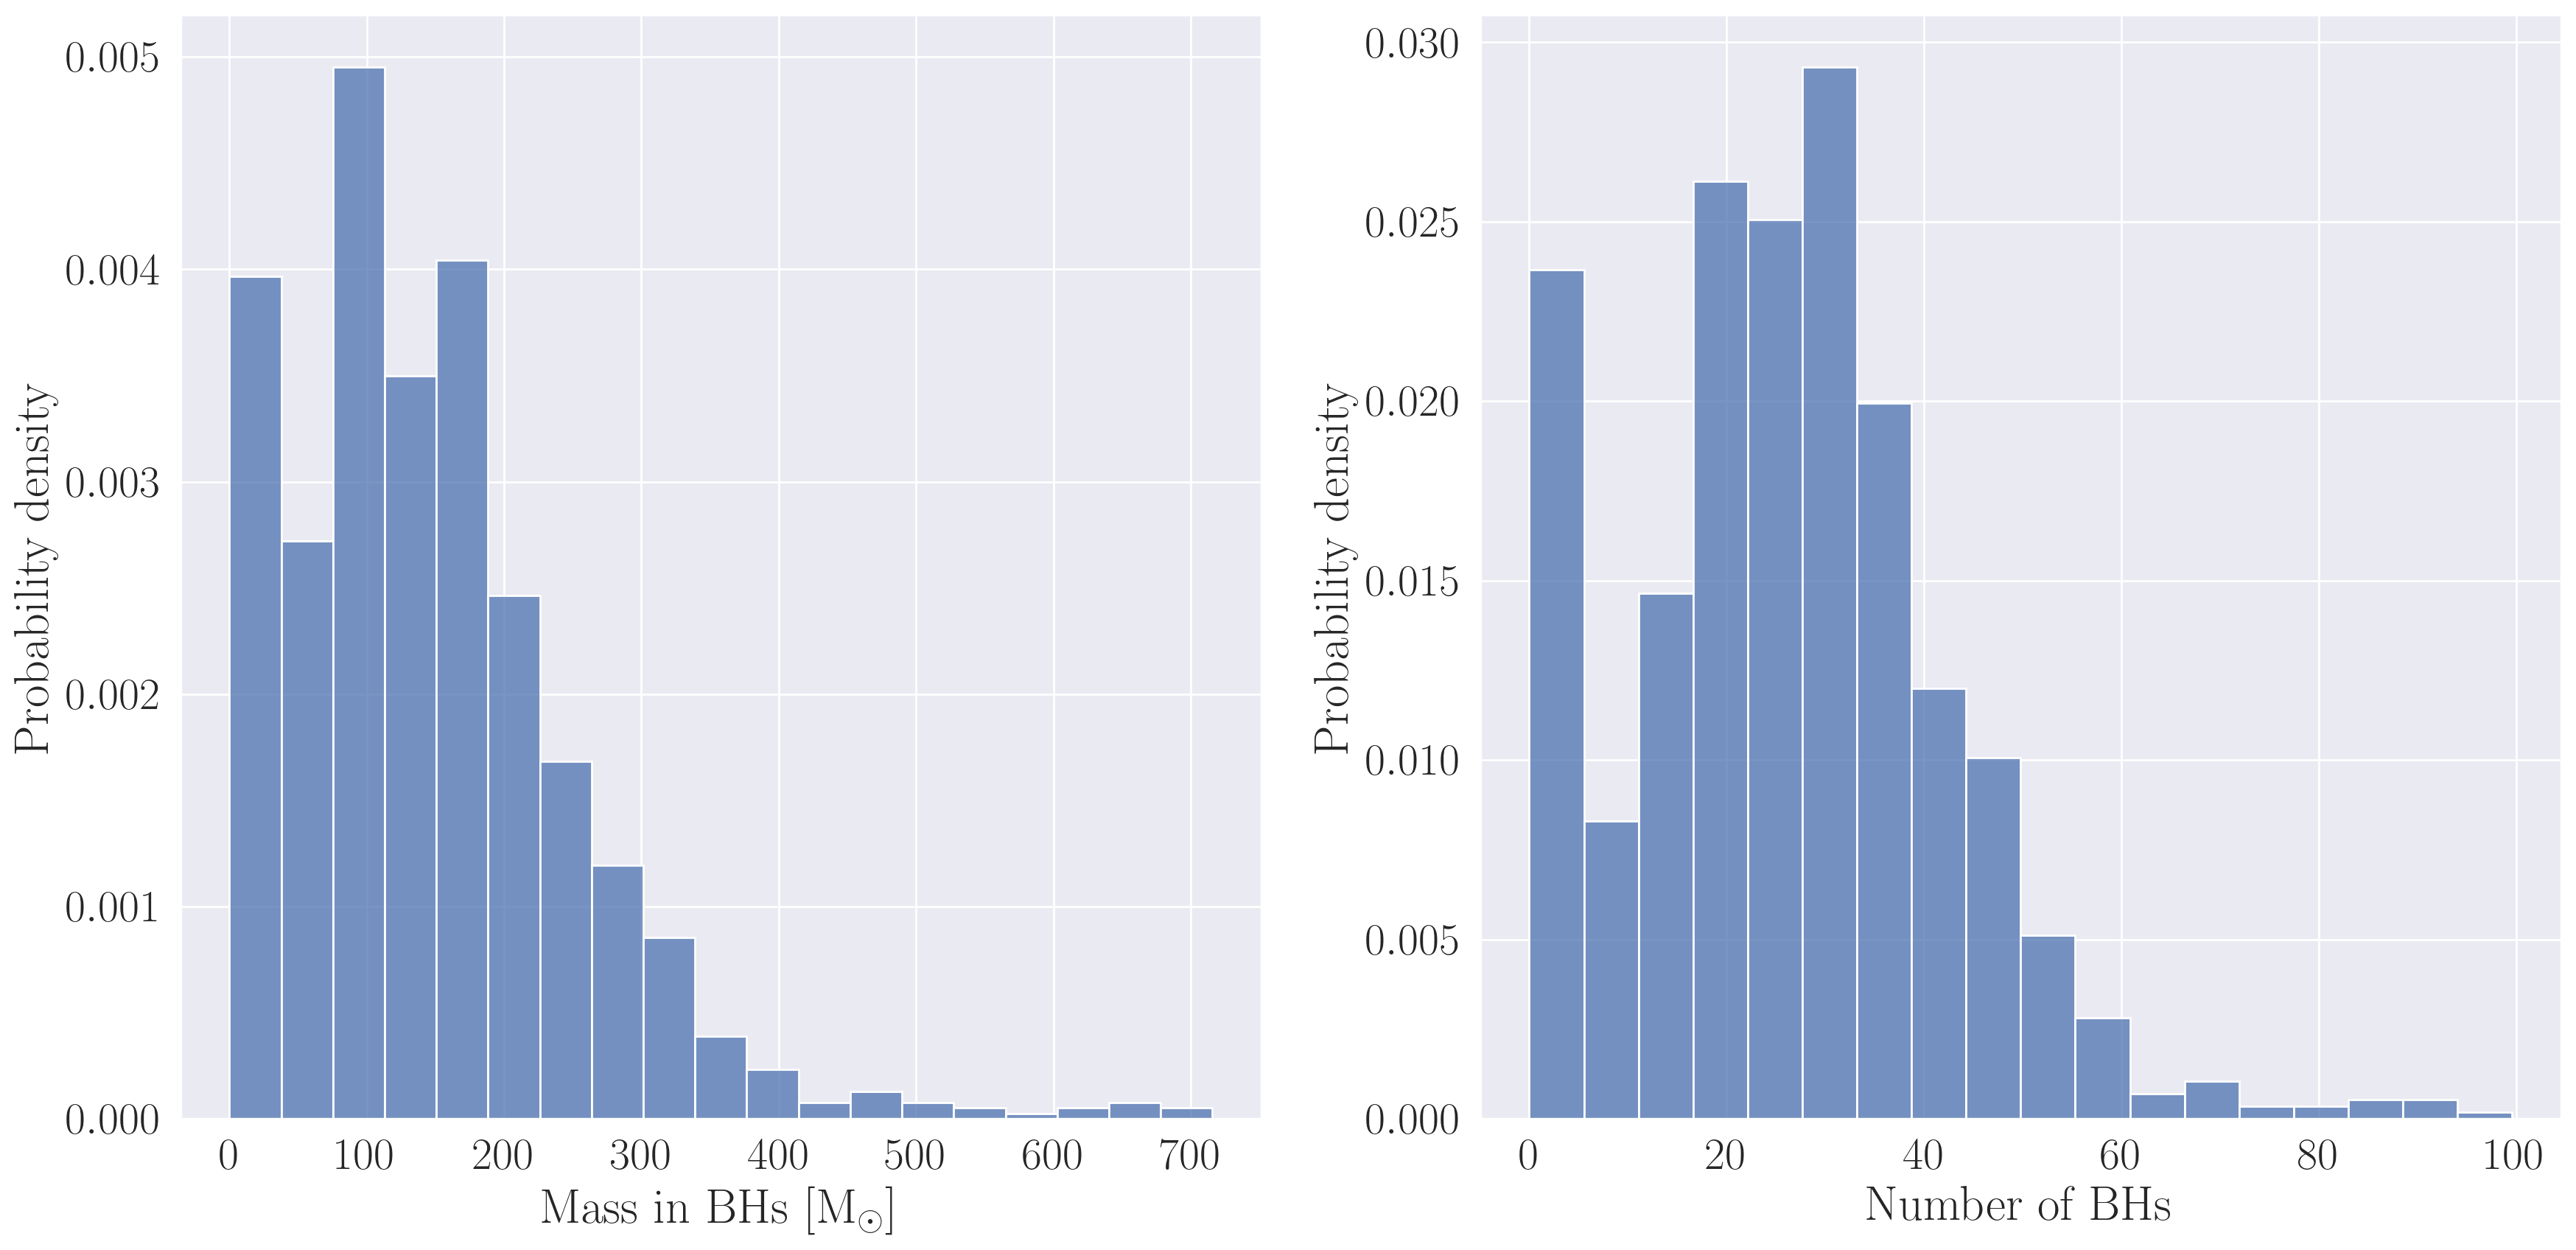
\includegraphics[width=0.8\textwidth]{figures/prev_nobin/BH_dists.png}
	\caption{BH distributions}
	\label{fig:prev_nobin_BH_dists}
\end{figure}


\subsection{Low Binary Fraction}
\ps{Describe the results for the low binary fraction model.}

In the low binary fraction case, the model is similar to the model without binaries. Maybe?

\ps{Figures with usual model quantities, also the binary mass histogram and the density profiles}


\begin{figure}
	\begin{center}
		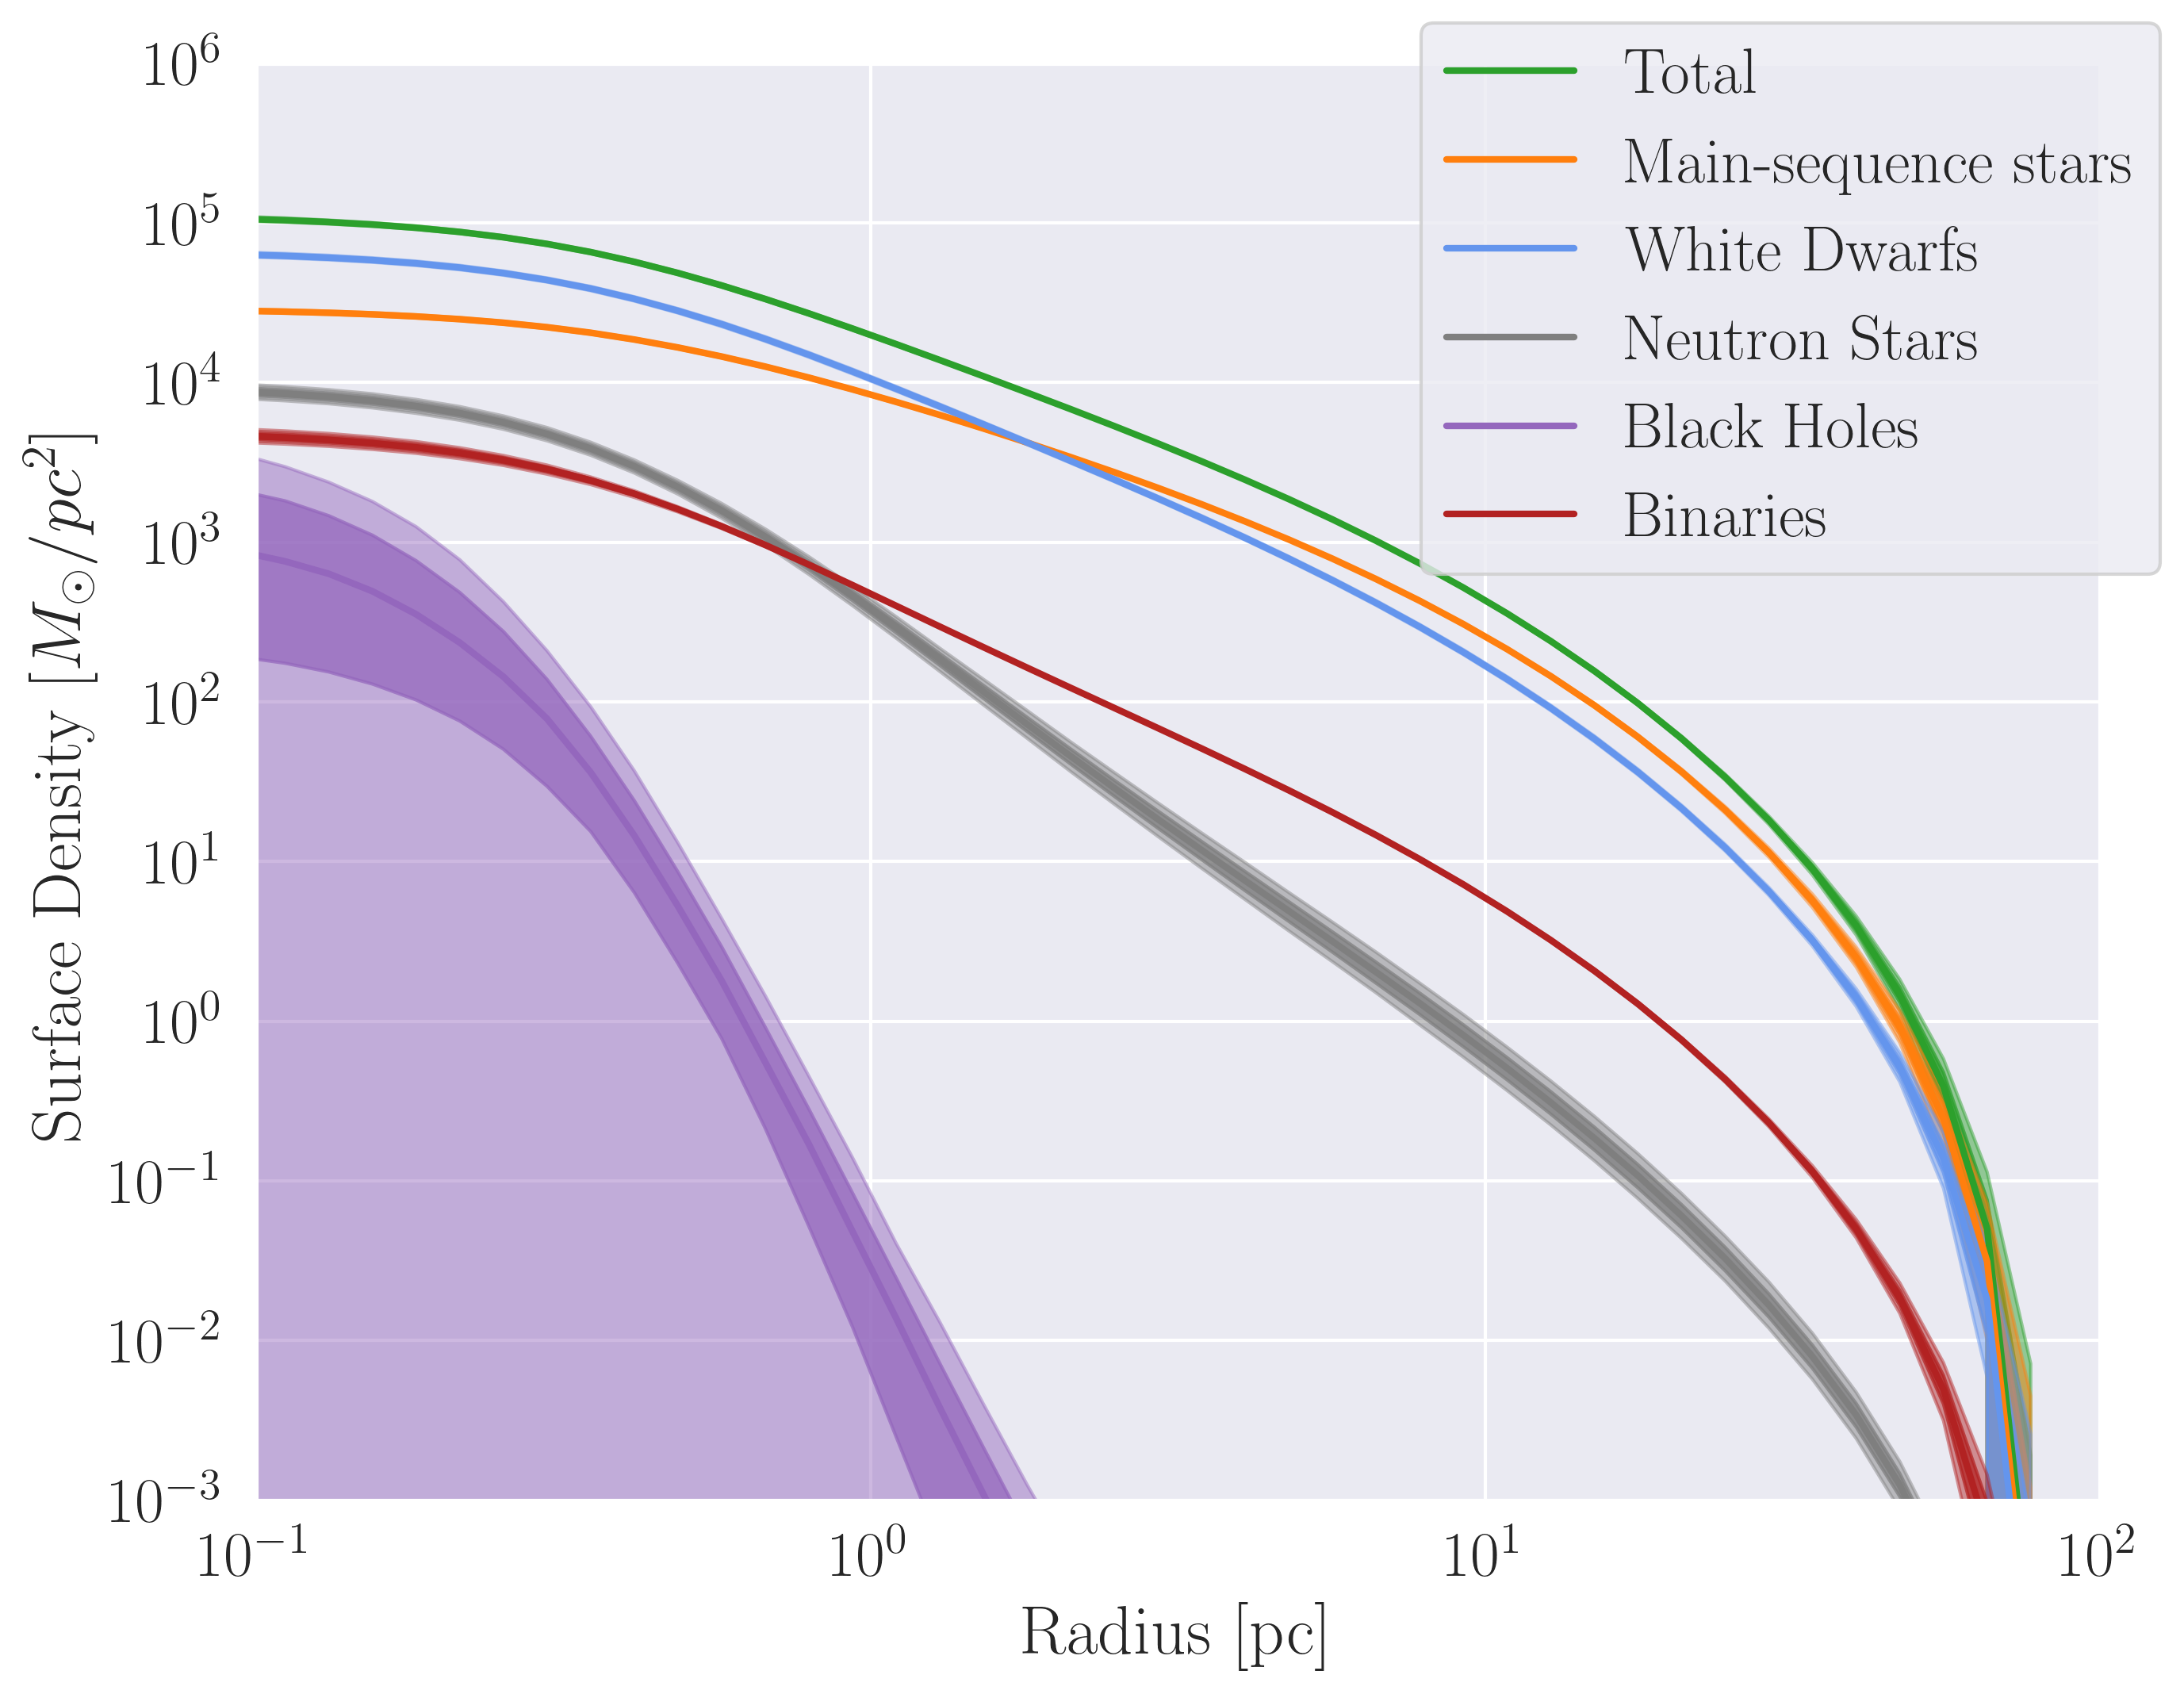
\includegraphics[width=0.9\textwidth]{figures/low_bin_model/surface_dens.png}
	\end{center}
	\caption{Density Profiles, do we prefer 3d density or surface density for this plot? Cumulative mass?}
	\label{fig:low_bin_model_densities}
\end{figure}


\begin{figure}
	\begin{center}
		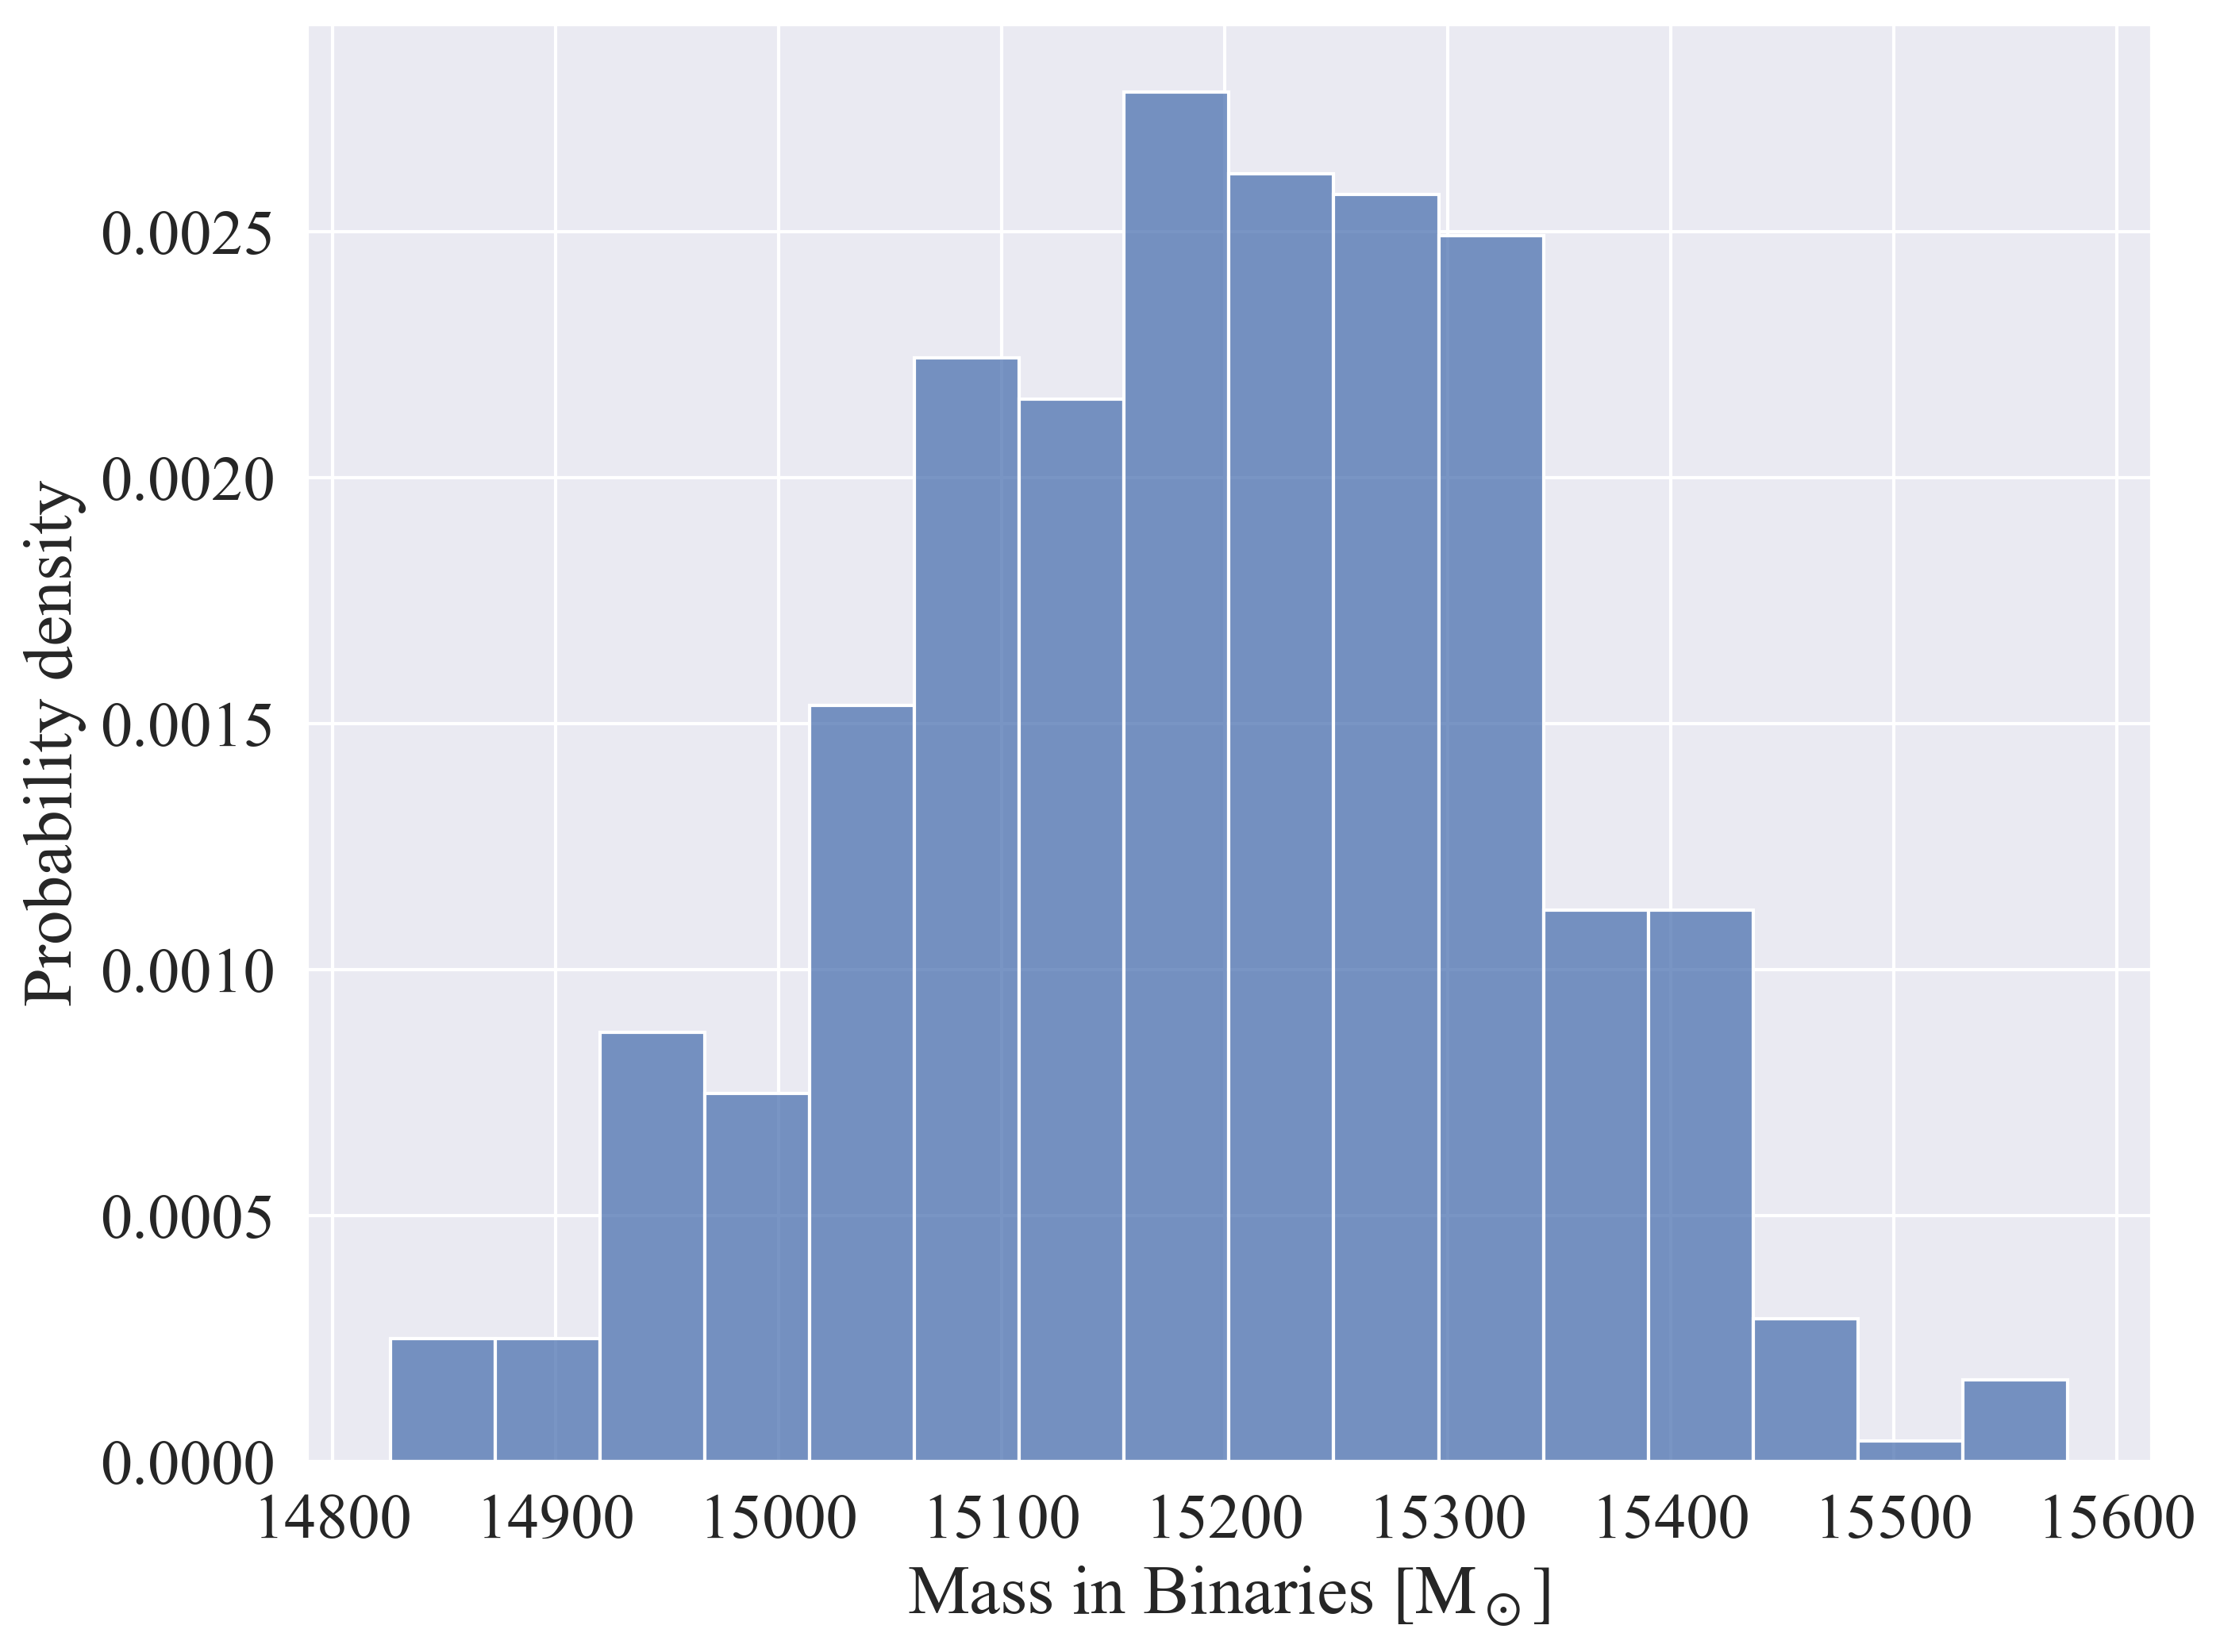
\includegraphics[width=0.9\textwidth]{figures/low_bin_model/binary_mass.png}
	\end{center}
	\caption{Total mass in binaries}
	\label{fig:low_bin_model_binary_mass}
\end{figure}

\begin{figure}
	\begin{center}
		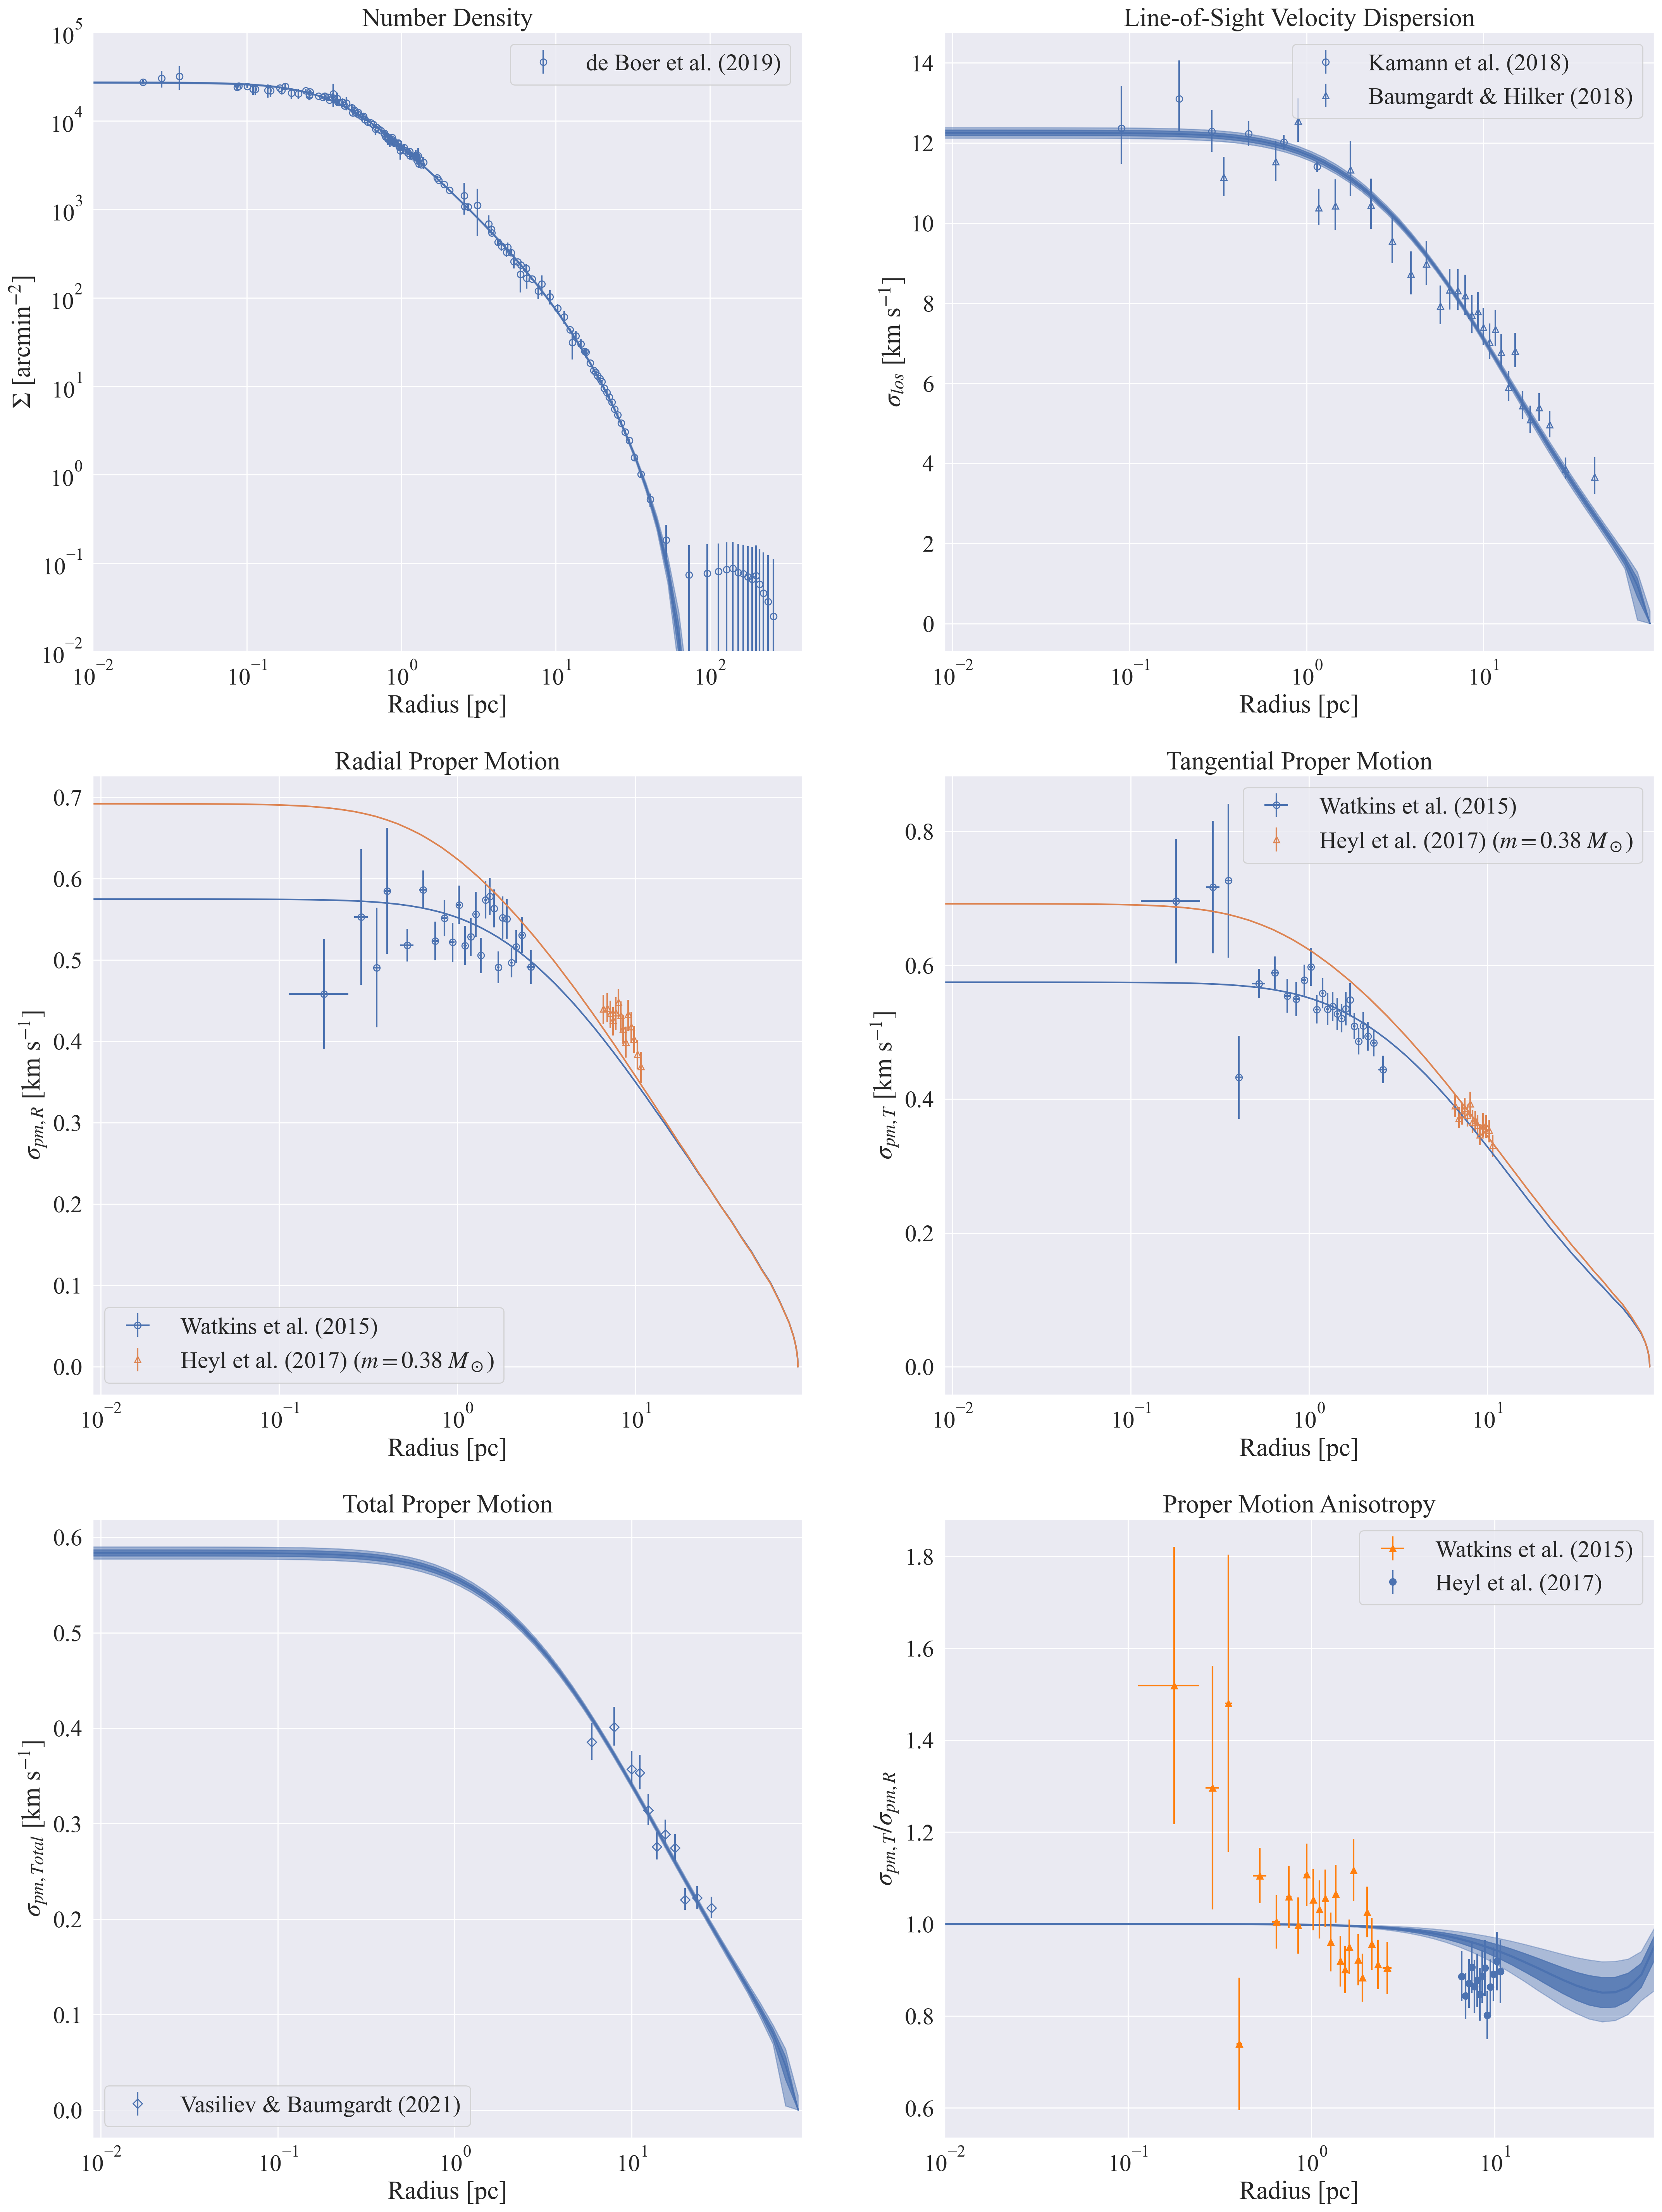
\includegraphics[width=0.9\textwidth]{figures/low_bin_model/obs_panel.png}
	\end{center}
	\caption{Observables}
	\label{fig:low_bin_model_obs_panel}
\end{figure}


\begin{figure}
	\begin{center}
		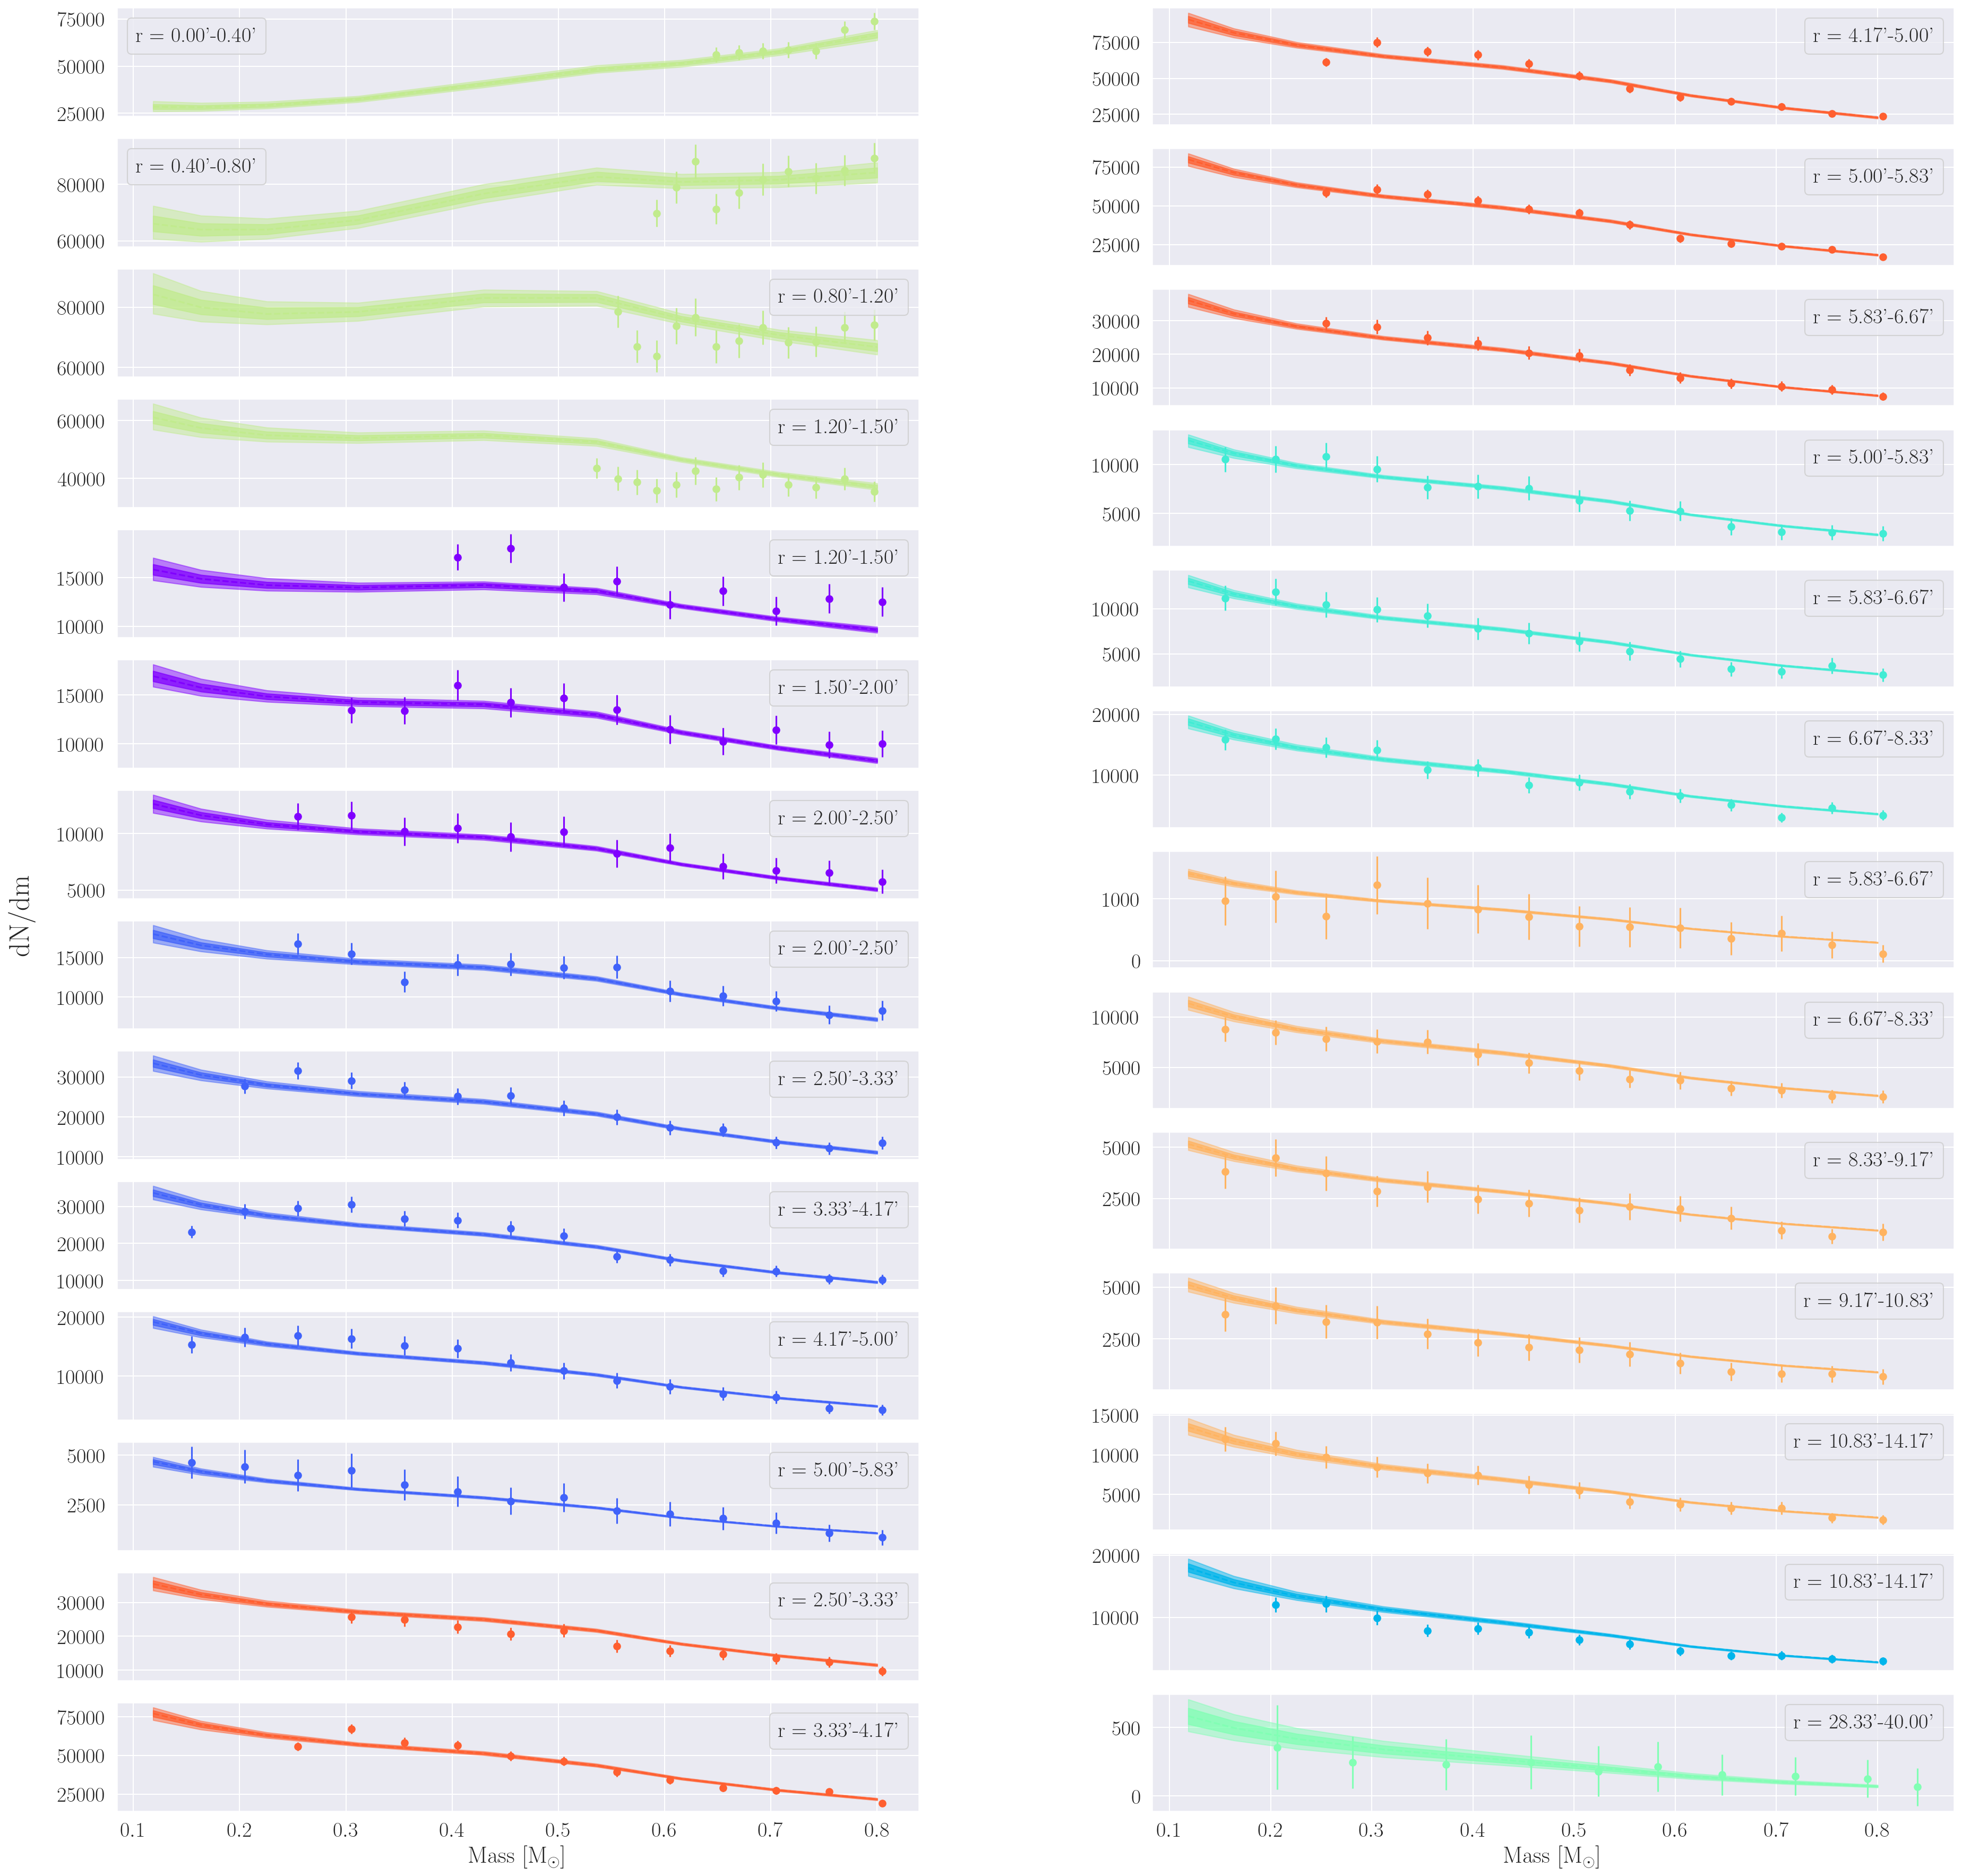
\includegraphics[width=\textwidth]{figures/low_bin_model/mass_fun.png}
	\end{center}
	\caption{Mass function}
	\label{fig:low_bin_model_mass_fun}
\end{figure}

\subsection{High Binary Fraction}
\ps{Describe the results for the high binary fraction model.}

\ps{Figures with usual model quantities, also the binary mass histogram and the density profiles}

\section{Discussion}

\subsection{The effects of the binaries}

Generally mimic a small population of remnants?


\subsection{Conclusion}

\ps{Implications for past/future work}

\ps{Do binaries in df models actually matter?}



\subsection{Future Work}

We're only looking at binaries in main sequence stars. WD binaries are probably a bigger effect, but
we have no data at all to constrain those quantities, so we ignore them. Maybe looking at N-body or
MC models could give some useful constraints.

Would be nice to look at a cluster where we know there is a larger binary population (NGC3201)and
fit with and without binaries to see what the effects are.